\subsection{Displacement approach}
\label{subsec:displacement_approach}

The displacement approach consists of assembling the global force vector $\mathbf{F}$ based on the `displacement method'.

In particular, if the structure is subjected to a distributed static load (as in the case of the gravity load), we know that the nodal forces on a single beam element can be computed as:

\begin{figure}[H]
    \centering
    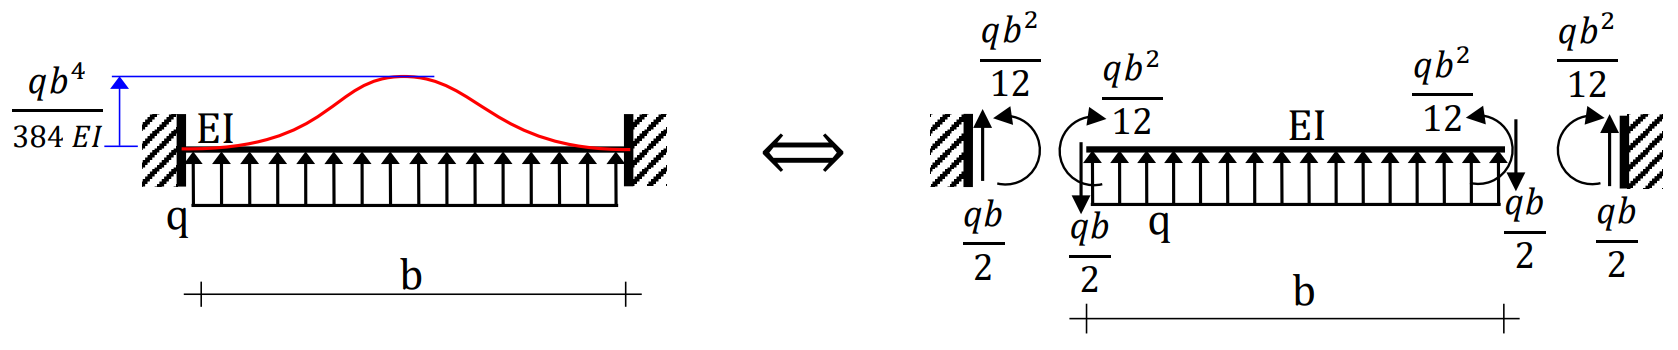
\includegraphics[width=0.9\textwidth]{img/displacement-method.png}
    \label{fig:displacement_method}
\end{figure}

From the figure above, we can obtain the coefficients needed to compute the equivalent forces due to a distributed force load along the element.

By using proper change in the reference system (by rotational matrices), it's possible to build the equivalent global force vector $\mathbf{F}$, which can be seen as the equivalent effect on the node of the structure due to the distributed load.

Finally, we can solve the equation of motion \ref{eq:static_responses} to obtain the displacements of the structure.

In \texttt{MATLAB}, the displacement approach can be implemented as follows:

\begin{lstlisting}[language=Matlab]

    % Displacement approach.
    F_global = zeros(3*nnod, 1);

    for ii = 1:nbeam

        [R, Q] = compute_rotational_matrices(gamma(ii));

        % Here we are negletting the possibility of a distributed momentum
        % load. Just distributed force loads are considered.
        elemental_distributed_load = R(1:2, 1:2)' * [0 -9.81 * m(ii)]';

        elemental_equivalent_nodal_load = [
            l(ii)/2 0
            0       l(ii)/2
            0       l(ii)^2/12
            l(ii)/2 0
            0       l(ii)/2
            0       -l(ii)^2/12
            ] * elemental_distributed_load;

        global_equivalent_nodal_load = Q * elemental_equivalent_nodal_load;

        F_global(incid(ii, :)) = F_global(incid(ii, :)) + global_equivalent_nodal_load;

    end

    X_gravity_displacement_approach = K_FF \ F_global(1:ndof);

\end{lstlisting}